\documentclass[main]{subfiles}

\begin{document}

\section{Experimentos y resultados con funciones de equivalencia de Dombi}\label{sec:resultadosmono}

% EXPERIMENTO 1
\subsection{Experimento 1: sustitución de la función REF por la función de Dombi en el algoritmo de maximización de la similitud}
\subsubsection{Explicación del experimento}
En este primer experimento pretendemos conocer cómo se pueden adaptar las funciones de Dombi que hemos descrito en \ref{def:dombi} para la sustitución de las funciones REF en la creación de los conjuntos difusos. Se han llevado a cabo experimentos con casi 30 imágenes. Entre todos estos experimentos, a continuación se presentan los más reelevantes. Para ello, se tomarán las imágenes que se muestran en la figura \ref{fig:imagenes}. Se muestran junto con sus histogramas así como las imágenes ya umbralizadas por parte de un experto (si existen).

En primer lugar, se procesarán las imágenes tomando el parámetro $w=1$ tanto para $x$ como para $y$. Después, y a la vista de unos resultados variables, se toma la determinación de ampliar el rango de pesos por lo que se prepara una prueba para los valores 0,1; 0,5; 0,75; 1; 1,25; 1,5; 2 y 5. Por último, para poder conocer la efectividad de todos estos resultados, son comparados contra el algoritmo de maximización de la similitud original tomando como equivalencia restringida todas las funciones que se han enumerado anteriormente en \ref{obs:funcionesref}, dándole especial importancia a la \mbox{$REF(x,y)=1-\abs{x-y}$} así como con todos los demás algoritmos explicados en el apartado \ref{sec:otrosalgoritmos} de la sección anterior.

Para poder conocer de forma empírica la diferencia entre dos imagenes segmentadas, se calcula para todas ellas el error cuadrático medio. Se puede expresar el error como
$$ECM(Q, Q') = \frac{\sum_{x=1}^N\sum_{y=1}^M \left(q(x,y)-q'(x,y)\right)^2}{N\cdot M}.$$

Para poder conocer cómo actua el algoritmo frente al ruido, se han preparado imágenes con ruido gausiano con media $\mu=0$ y varianza $\sigma^2 = 0,01$. También, se han preparado con ruido impulsivo, de `de sal y pimienta' con densidad de probabilidad del ruido $d=0,05$ y $d=0,2$. Se presentan las imágenes ya tratadas en la figura \ref{fig:imagenesruido}. Por otra parte, se prueba a ver cómo resiste el algoritmo con imágenes de bajo y alto contraste.

\begin{figure}
\centering
    \subfigure[`Silla']
    {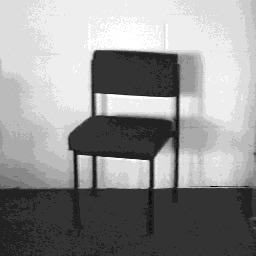
\includegraphics[width=0.22\textwidth]{img/orig/chair.jpg}}\quad
    \subfigure[Histograma]
    {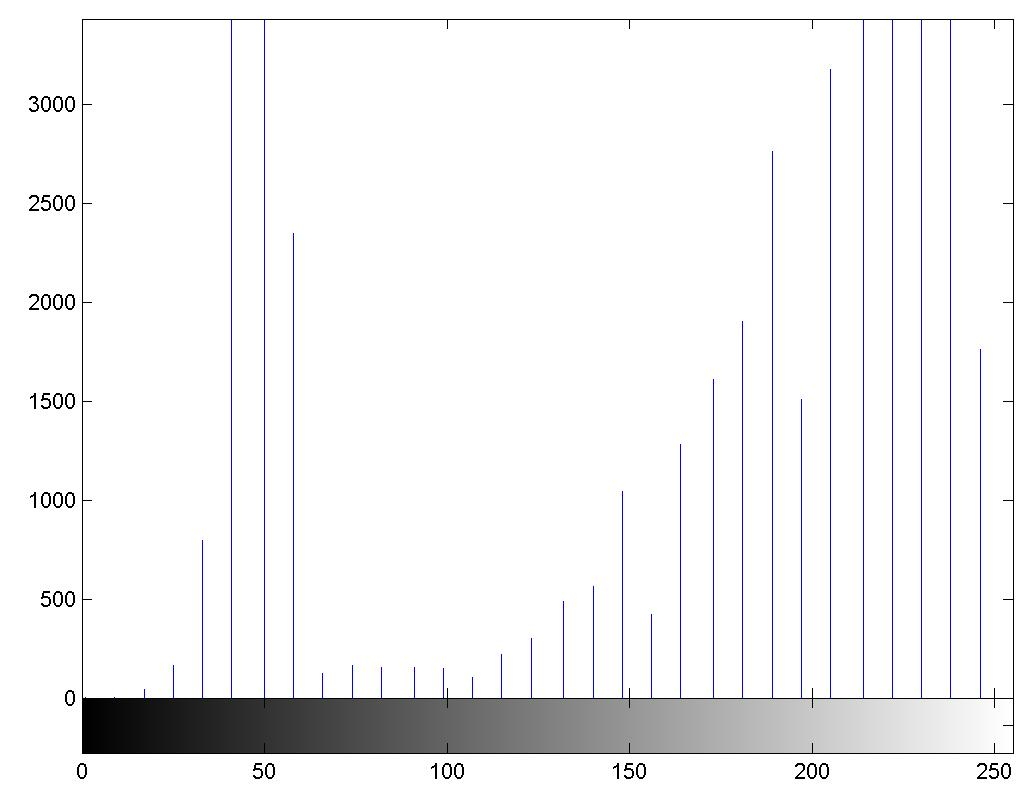
\includegraphics[width=0.28\textwidth]{img/hist/hist-chair.jpg}}\\
    \subfigure[`Bloques']
    {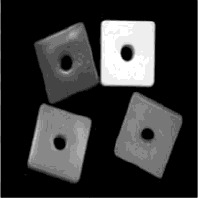
\includegraphics[width=0.22\textwidth]{img/orig/block.jpg}}\quad
    \subfigure[Umbralización del experto.]
    {
\includegraphics[width=0.22\textwidth]{img/orig/blockbin.jpg}}\quad
    \subfigure[Histrograma]
    {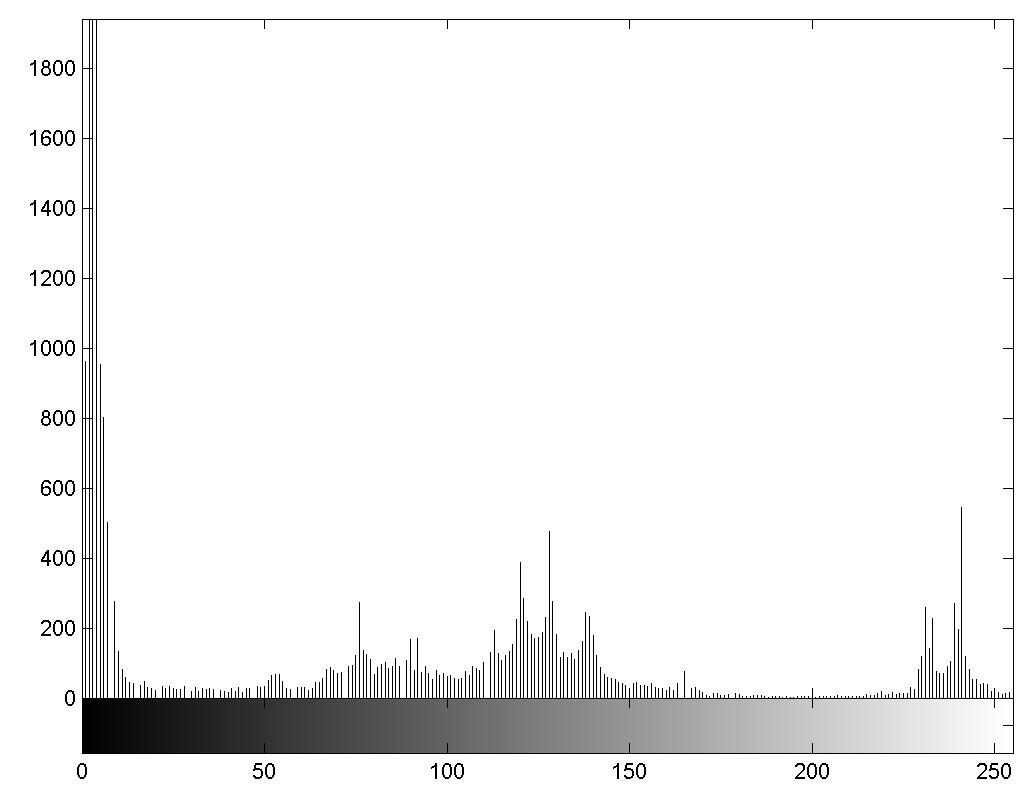
\includegraphics[width=0.28\textwidth]{img/hist/hist-block.jpg}}\\
    \subfigure[`Engranaje']
    {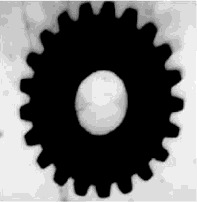
\includegraphics[width=0.22\textwidth]{img/orig/02.jpg}}\quad
    \subfigure[Umbralización del experto.]
    {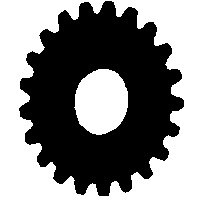
\includegraphics[width=0.22\textwidth]{img/orig/02bin.jpg}}\quad
    \subfigure[Histrograma]
    {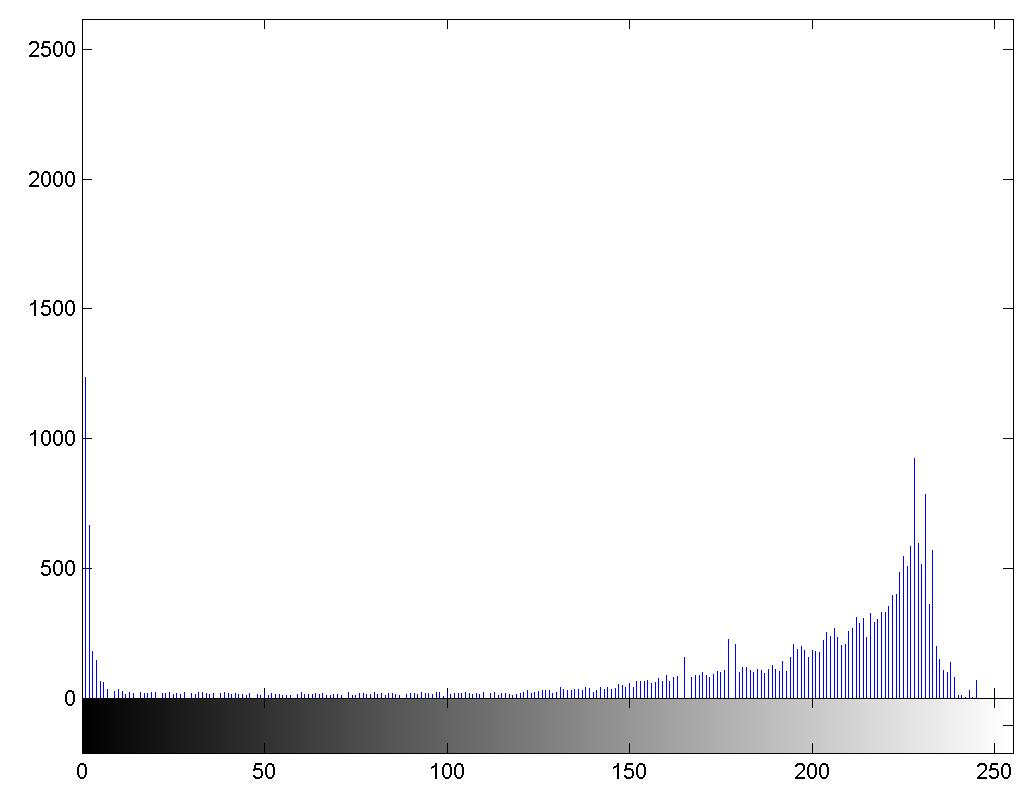
\includegraphics[width=0.28\textwidth]{img/hist/hist-02.jpg}}\\
    %\subfigure[`Piedras']
    %{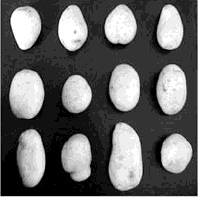
\includegraphics[width=0.22\textwidth]{img/orig/04.jpg}}\quad
    %\subfigure[Umbralización del experto.]
    %{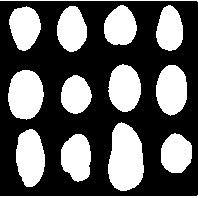
\includegraphics[width=0.22\textwidth]{img/orig/04bin.jpg}}\quad
    %\subfigure[Histrograma]
    %{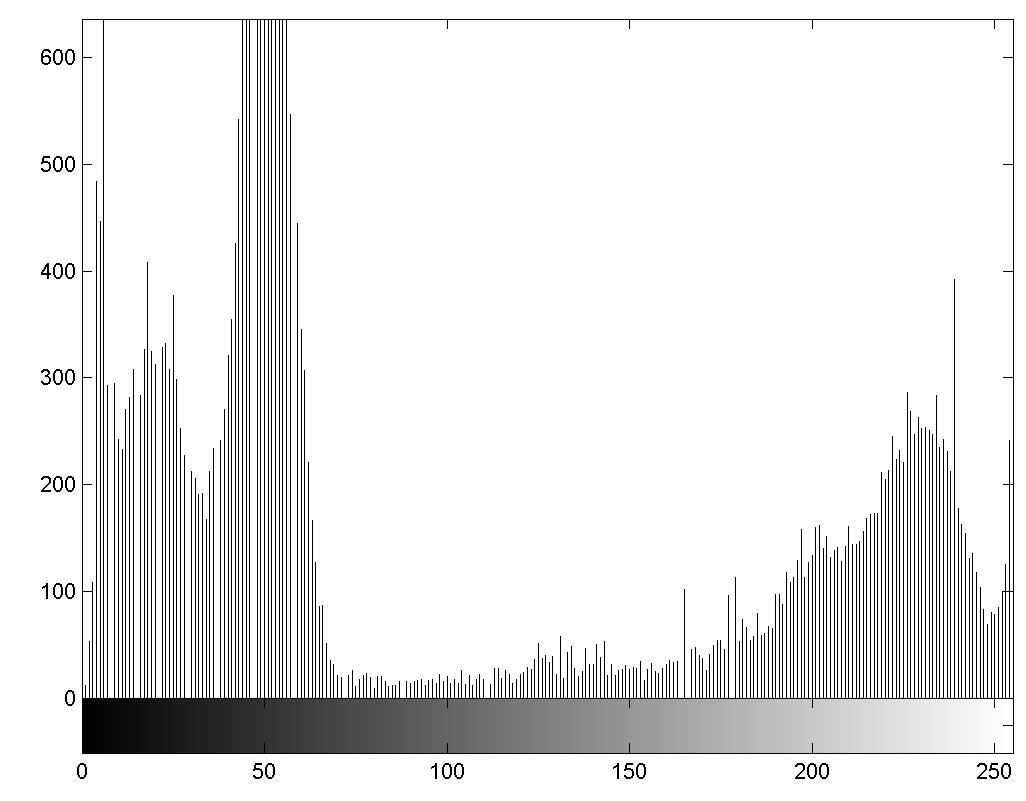
\includegraphics[width=0.28\textwidth]{img/hist/hist-04.jpg}}\\
    \subfigure[`Letras']
    {
\includegraphics[width=0.22\textwidth]{img/orig/09.jpg}}\quad
    \subfigure[Umbralización del experto.]
    {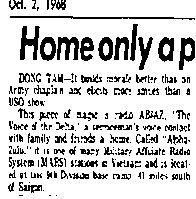
\includegraphics[width=0.22\textwidth]{img/orig/09bin.jpg}}\quad
    \subfigure[Histrograma]
    {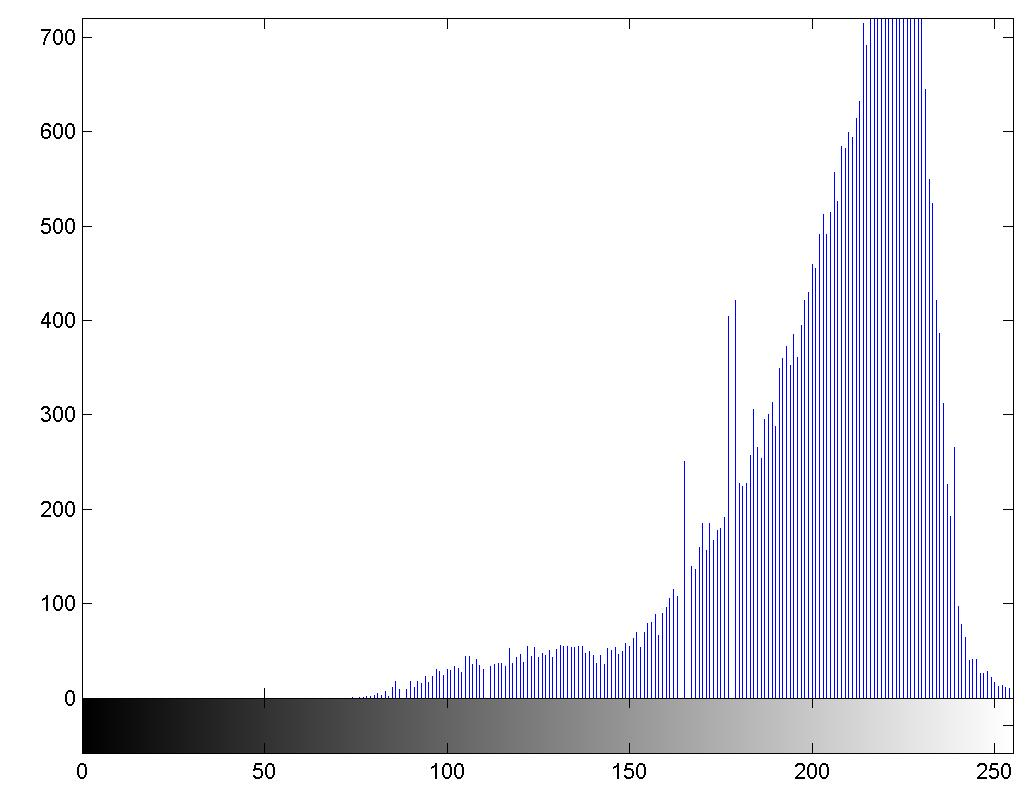
\includegraphics[width=0.28\textwidth]{img/hist/hist-09.jpg}}
    \subfigure[`Sombra']
    {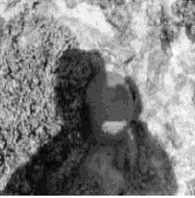
\includegraphics[width=0.22\textwidth]{img/orig/07.jpg}}\quad
    \subfigure[Umbralización del experto.]
    {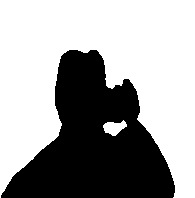
\includegraphics[width=0.22\textwidth]{img/orig/07bin.jpg}}\quad
    \subfigure[Histrograma]
    {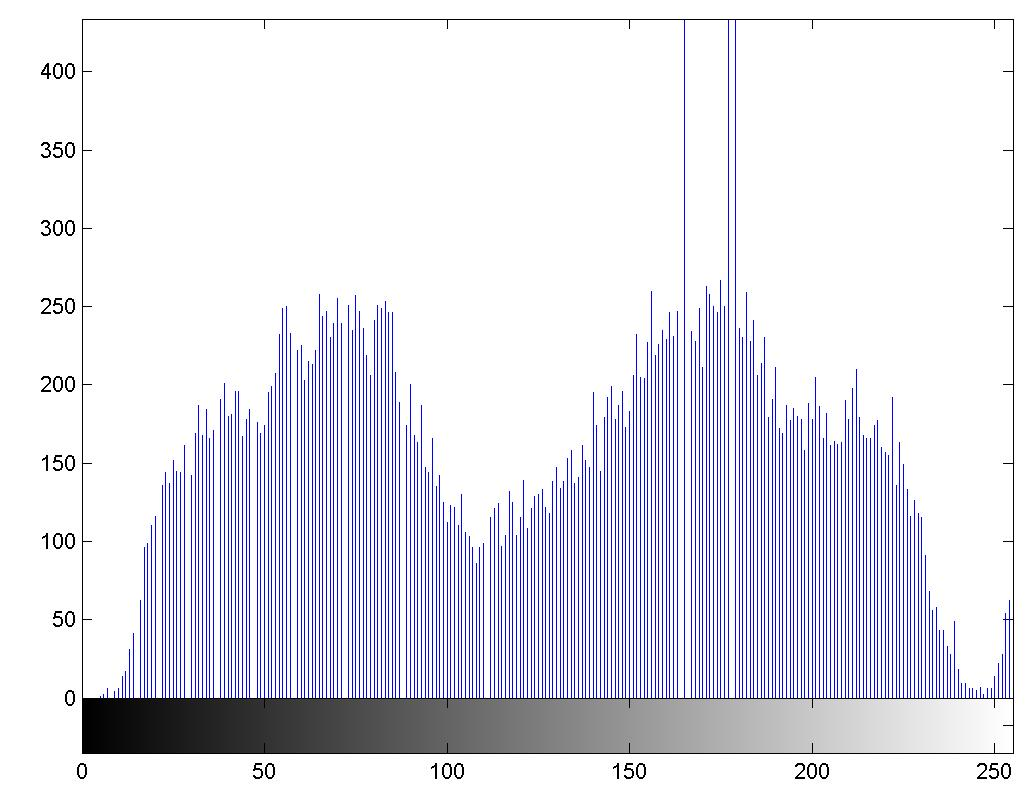
\includegraphics[width=0.28\textwidth]{img/hist/hist-07.jpg}}
    \caption{Imágenes utilizadas en el experimento 1 y siguientes.}
    \label{fig:imagenes}
\end{figure}

%\REV{faltan histogramas figura \ref{fig:sillaconruido}} Solucionado
%\REV{incluir figura con maximo contraste}
%\begin{figure}
%\centering
%    \subfigure[Muy alto contraste]
%    {\includegraphics[width=0.22\textwidth]{img/orig/chairmuyacon.jpg}}\quad
%    \subfigure[Alto contraste]
%    {\includegraphics[width=0.22\textwidth]{img/orig/chairacon.jpg}}\quad
%    \subfigure[Bajo contraste]
%    {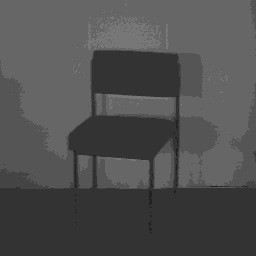
\includegraphics[width=0.22\textwidth]{img/orig/chairbcon.jpg}}\quad
%    \subfigure[Muy bajo contraste]
%    {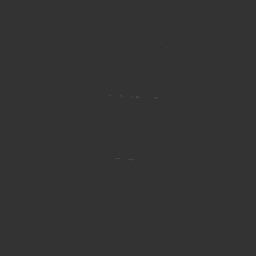
\includegraphics[width=0.22\textwidth]{img/orig/chairmuybcon.jpg}}
%    \caption{Imágenes con ruido utilizadas en el experimento 1 y siguientes.}
%    \label{fig:sillaconcontraste}
%\end{figure}

\subsubsection{Resultados}
En la tabla \ref{tab:resultexp1dombi} se pueden apreciar los resultados para la umbralización de cada una de las imágenes y diferentes $w$. Se dispone, también de la tabla \ref{tab:resultexp1otros} donde se expresan los umbrales para otros algoritmos. En la comparación de ambas tablas se obtiene un resultado claro, el parámetro $w$ influye de forma determinante en la segmentación de las imágenes. Así, por ejemplo, en el caso de la `silla' $w=1$ es una opción totalmente acertada mientras que para para las `letras' habría que doblar el valor para obtener una umbralización igual de buena en comparación con los otros métodos.

\begin{table}
\centering
\begin{tabular}{c||c|c|c|c|c}
$\mathbf{w}$    &\bb Silla&\bb Bloques&\bb Engranaje&\bb Letras&\bb Sombra\\\hline\hline
$\mathbf{0,1}$  &   218   &    255    &     250     &   142    &   200  \\\hline
$\mathbf{0,5}$  &   226   &    255    &     250     &    39    &   230  \\\hline
$\mathbf{0,75}$ &    95   &    119    &     115     &   103    &   111  \\\hline
$\mathbf{1}$    &   127   &    123    &     137     &   160    &   125  \\\hline
$\mathbf{1,25}$ &    70   &     97    &      96     &    80    &    91  \\\hline
$\mathbf{1,5}$  &    45   &     79    &      0      &    39    &    64  \\\hline
$\mathbf{2}$    &   144   &     76    &     138     &   197    &    96  \\\hline
$\mathbf{5}$    &   218   &     31    &      59     &   216    &   219  \\\hline
\end{tabular}
\caption{Umbrales para cada imagen con la función de Dombi y diferentes $w$.\label{tab:resultexp1dombi}}
\end{table}

\begin{table}
\centering
\begin{tabular}{c||c|c|c|c|c}
                                                  &\bb Silla&\bb Bloques&\bb Engranaje&\bb Letras&\bb Sombra\\\hline\hline
\bb Alg. 1 con $\mathbf{REF_1=1-\abs{x-y}}$         &   127   &     79    &     104     &   187    &   123  \\\hline
\bb Alg. 1 con $\mathbf{REF_1=1-\abs{x-y}^2}$       &   127   &     97    &     140     &   179    &   126  \\\hline
\bb Alg. 1 con $\mathbf{REF_1=1-\abs{x-y}^{0.5}}$   &   119   &     47    &      84     &   200    &   121  \\\hline
\bb Alg. 1 con $\mathbf{REF_1=(1-\abs{x-y})^2}$     &   127   &     70    &     105     &   190    &   123  \\\hline
\bb Alg. 1 con $\mathbf{REF_1=(1-\abs{x-y})^{0.5}}$ &   127   &     82    &     104     &   186    &   124  \\\hline
\bb U. Global                                       &   130   &     79    &     105     &   187    &   124  \\\hline
\bb U. de Otsu                                      &   123   &     79    &     104     &   187    &   123  \\\hline
\bb Máx. la entropía de Renyi                       &   170   &     32    &     131     &   160    &   135  \\\hline
\end{tabular}
\caption{Umbrales para cada imagen con otras versiones de algoritmos.\label{tab:resultexp1otros}}
\end{table}

Por otra parte, cabe destacar que este resultado se ha obtenido en un tiempo de computación de alrededor de 0,0025 segundos, tanto para la versión con función de Dombi como para la de REF. Con la intención de que el lector pueda juzgar adecuadamente estos resutlados, se presentan los resultados, en forma gráfica, para aquellos valores de $w$ más reelevantes de forma gráfica en la tabla \ref{tab:resultexp1imagenesdombi}. Se facilita la posibilidad de poder compararlo directamente con el algoritmo original. Además, se dispone en el apéndice \ref{cap:anexotrassegmentaciones}, en las tablas \ref{tab:otrassegmentacionesruido} y \ref{tab:otrassegmentaciones}, la umbralización de las imágenes con otros algoritmos para que se pueda llevar a cabo también la comparación.

\begin{table}
\centering
\begin{tabular}{c||c|c|c}
$\mathbf{REF_1=1-\abs{x-y}}$ & $\mathbf{w=0,75}$ &\bb $\mathbf{w=1}$ &\bb $\mathbf{w=1,25}$\\\hline\hline
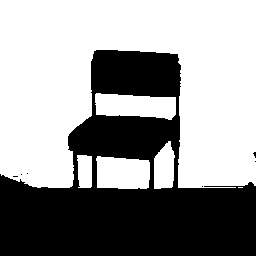
\includegraphics[width=0.2\textwidth]{img/res/e1a/alg1tipo1-chair.jpg} &
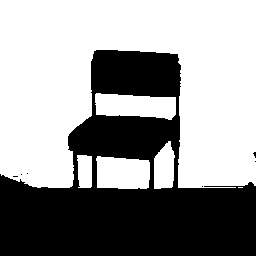
\includegraphics[width=0.2\textwidth]{img/res/e1a/alg1tipo6-chair.jpg} &
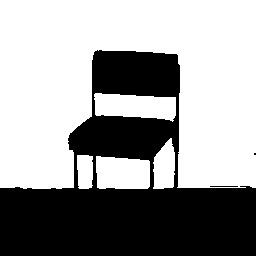
\includegraphics[width=0.2\textwidth]{img/res/e1a/alg1tipo6d0.75-chair.jpg} &
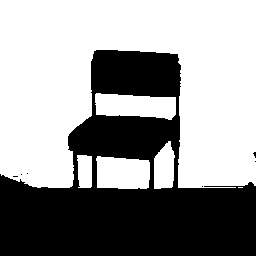
\includegraphics[width=0.2\textwidth]{img/res/e1a/alg1tipo6d1.25-chair.jpg} \\
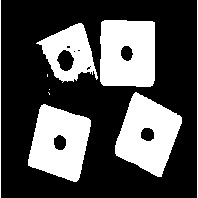
\includegraphics[width=0.2\textwidth]{img/res/e1a/alg1tipo1-block.jpg} &
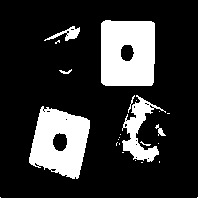
\includegraphics[width=0.2\textwidth]{img/res/e1a/alg1tipo6-block.jpg} &
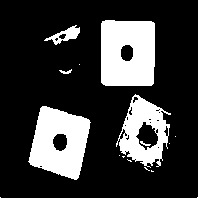
\includegraphics[width=0.2\textwidth]{img/res/e1a/alg1tipo6d0.75-block.jpg} &
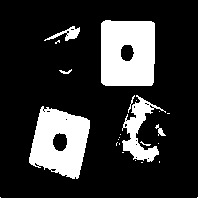
\includegraphics[width=0.2\textwidth]{img/res/e1a/alg1tipo6d1.25-block.jpg} \\
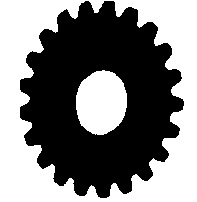
\includegraphics[width=0.2\textwidth]{img/res/e1a/alg1tipo1-02.jpg} &
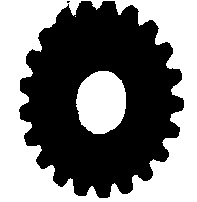
\includegraphics[width=0.2\textwidth]{img/res/e1a/alg1tipo6-02.jpg} &
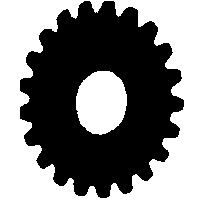
\includegraphics[width=0.2\textwidth]{img/res/e1a/alg1tipo6d0.75-02.jpg} &
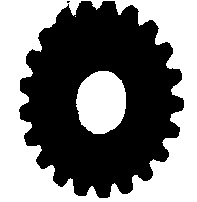
\includegraphics[width=0.2\textwidth]{img/res/e1a/alg1tipo6d1.25-02.jpg} \\
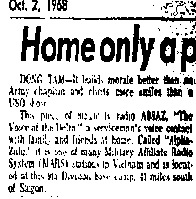
\includegraphics[width=0.2\textwidth]{img/res/e1a/alg1tipo1-09.jpg} &
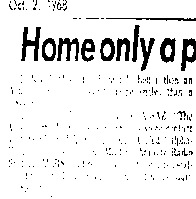
\includegraphics[width=0.2\textwidth]{img/res/e1a/alg1tipo6-09.jpg} &
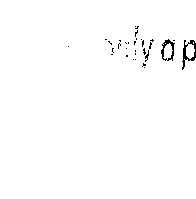
\includegraphics[width=0.2\textwidth]{img/res/e1a/alg1tipo6d0.75-09.jpg} &
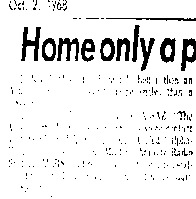
\includegraphics[width=0.2\textwidth]{img/res/e1a/alg1tipo6d1.25-09.jpg} \\
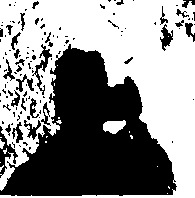
\includegraphics[width=0.2\textwidth]{img/res/e1a/alg1tipo1-07.jpg} &
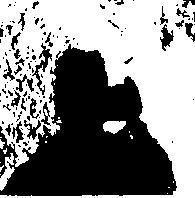
\includegraphics[width=0.2\textwidth]{img/res/e1a/alg1tipo6-07.jpg} &
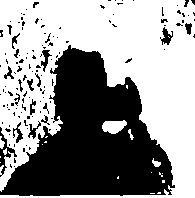
\includegraphics[width=0.2\textwidth]{img/res/e1a/alg1tipo6d0.75-07.jpg} &
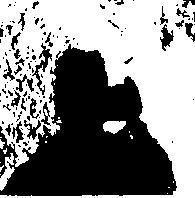
\includegraphics[width=0.2\textwidth]{img/res/e1a/alg1tipo6d1.25-07.jpg} \\\hline
\end{tabular}
\caption{Resultado de las segmentaciones para el algoritmo con REF y Dombi con varios $w = \{0,75; 1; 1,25\}$.\label{tab:resultexp1imagenesdombi}}
\end{table}

Para poder comprobar y comparar formalmente todos los resultados, se calcula el error cuadrático medio para las imágenes. En concreto, se hace con todas las versiones obtenidas con otros los algoritmos presentados sin obtener ningún resultado reelevante. Se presentan en la tabla \ref{tab:erroresexp1dombi}, la comparación que se hace entre las segmentaciones que se obtienen con varias $w$ y la imagen umbralizada de forma exacta por un experto, resultados que se hacen más interesantes que los anteriores. De nuevo, de esta tabla se desprende de que en función de la imagen que se tome, el parámetro $w$ para obtener una mejor umbralización.

\begin{table}
\centering
\begin{tabular}{c||c|c|c|c}
$\mathbf{w}$                    &\bb Bloques&\bb Engranaje&\bb Letras&\bb Sombra\\\hline\hline
\bb Alg. 1 con $\mathbf{0,75}$  &   43,3750  &   33,0080   &   33,3617   &   59,2420  \\\hline
\bb Alg. 1 con $\mathbf{1}$     &   49,8760  &   36,3914   &   29,6418   &   52,0672  \\\hline
\bb Alg. 1 con $\mathbf{1,25}$  &   50,0241  &   32,0153   &   31,0001   &   55,0322  \\\hline
\end{tabular}
\caption{Errores para las imágenes con ruido con otras versiones de algoritmos.\label{tab:erroresexp1dombi}}
\end{table}


%Con ruido
Con la intención de poder llevar a cabo experimentos sobre imágenes con ruido, se crean estas de forma sintética, tal y como se ha presentando en la sección \ref{sec:ruido}. Se pueden ver los resultados sobre la imagen `silla', y sus histogramas, en la figura \ref{fig:imagenesruido}.

\begin{figure}
\centering
    \subfigure[Ruido gausiano]
    {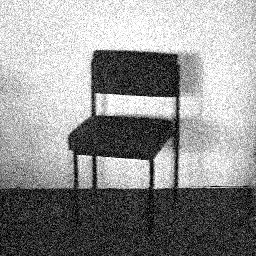
\includegraphics[width=0.25\textwidth]{img/orig/chairga.jpg}}\quad
    \subfigure[Ruido `sal y pimienta' con $p=0,05$]
    {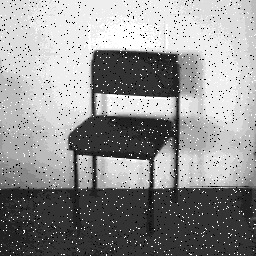
\includegraphics[width=0.25\textwidth]{img/orig/chairs&p005.jpg}}\quad
    \subfigure[Ruido `sal y pimienta' con $p=0,2$]
    {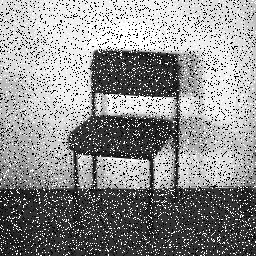
\includegraphics[width=0.25\textwidth]{img/orig/chairs&p020.jpg}}
    \subfigure[Histograma de ruido gausiano]
    {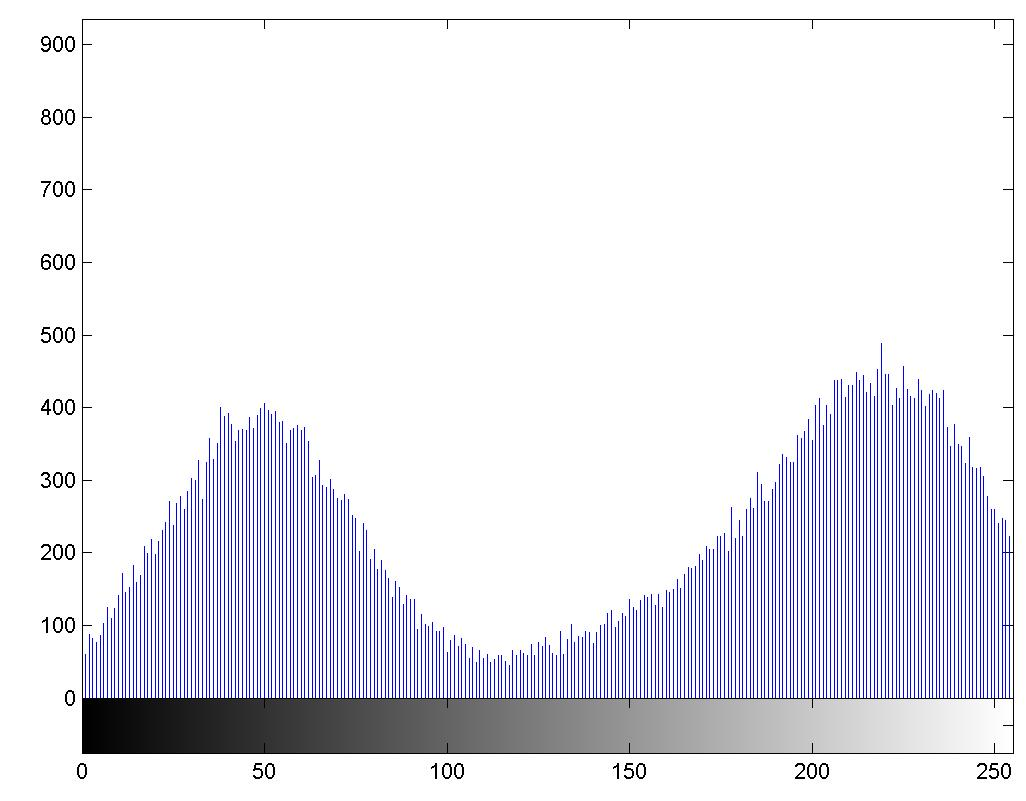
\includegraphics[width=0.3\textwidth]{img/hist/hist-chairga.jpg}}\quad
    \subfigure[Histograma de ruido `sal y pimienta' con $p=0,05$]
    {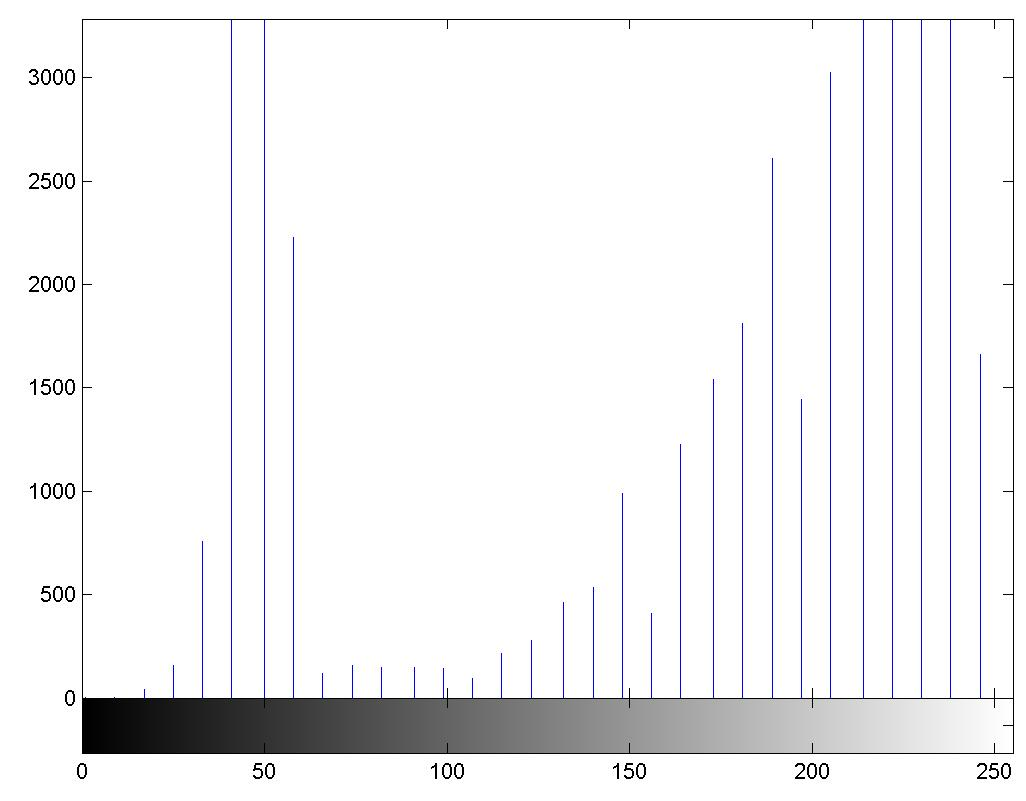
\includegraphics[width=0.3\textwidth]{img/hist/hist-chairsp005.jpg}}\quad
    \subfigure[Histograma de ruido `sal y pimienta' con $p=0,2$]
    {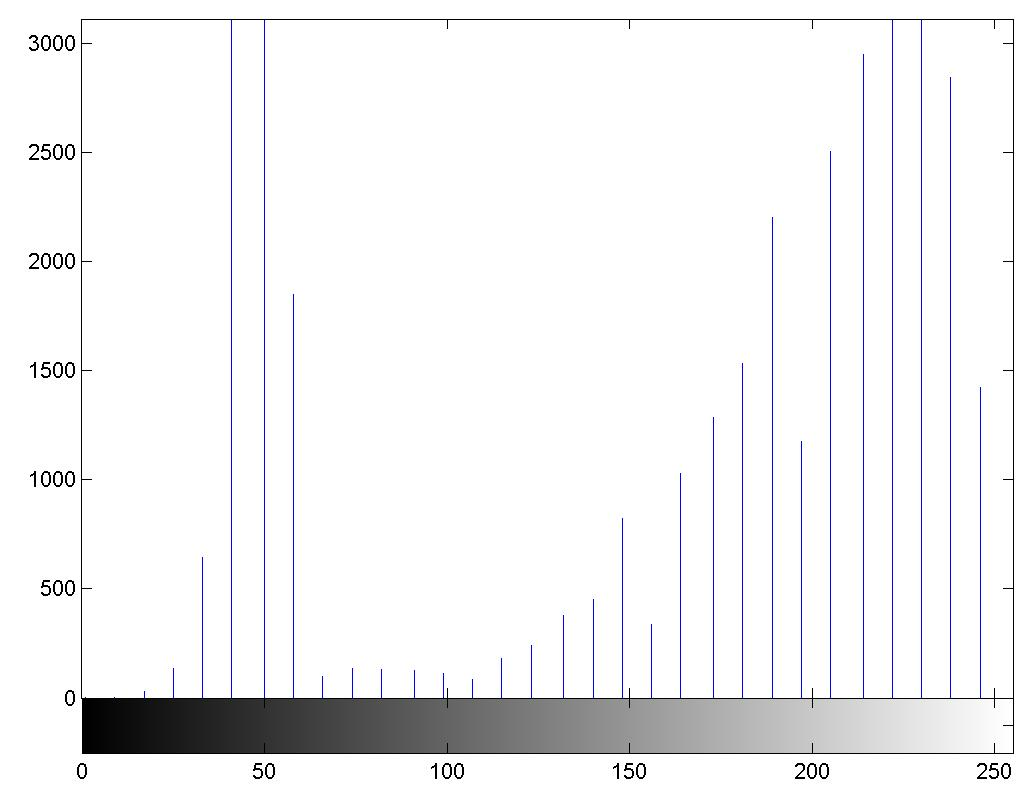
\includegraphics[width=0.3\textwidth]{img/hist/hist-chairsp020.jpg}}
    \caption{Imágenes con ruido utilizadas en el experimento 1 y siguientes.}
    \label{fig:imagenesruido}
\end{figure}

Los umbrales que se han obtenido se expresan en la tabla \ref{tab:resultexp1ruido}. Comparándola de nuevo con otros algoritmos (tablas \ref{tab:resultexp1ruidootros}), se puede apreciar que se pueden obtener resultados similiares también e, igualmente, que el parámetro $w$ es decisivo para diferentes imágenes. Es curioso comprobar el hecho de que con la misma $w$ se obtienen resultados similares en comparación con los umbrales de la versión original con REF.

\begin{table}
\centering
\begin{tabular}{c||c|c|c}
           &\bb R. gausiano&\bb R. impulsivo 0.05&\bb R. impulsivo 0.2\\\hline\hline
$\mathbf{0,1}$  &   219   &    226    &     226     \\\hline
$\mathbf{0,5}$  &   234   &    226    &     242     \\\hline
$\mathbf{0,75}$ &    99   &     95    &      95     \\\hline
$\mathbf{1}$    &   128   &    127    &     127     \\\hline
$\mathbf{1,25}$ &    74   &     70    &      62     \\\hline
$\mathbf{1,5}$  &    35   &     45    &      37     \\\hline
$\mathbf{2}$    &   147   &    136    &     127     \\\hline
$\mathbf{5}$    &   226   &    218    &     226     \\\hline
\end{tabular}
\caption{Umbrales para las imágenes con ruido con la función de Dombi y diferentes valores de $w$.\label{tab:resultexp1ruido}}
\end{table}


\begin{table}
\centering
\begin{tabular}{c||c|c|c}
                          &\bb R. gausiano&\bb R. impulsivo 0.05&\bb R. impulsivo 0.2\\\hline\hline
\bb Alg. 1 con $\mathbf{REF_1=1-\abs{x-y}}$             &   132   &    127    &     127     \\\hline
\bb Alg. 1 con $\mathbf{REF_1=1-\abs{x-y}^2}$           &   131   &    127    &     127     \\\hline
\bb Alg. 1 con $\mathbf{REF_1=1-\abs{x-y}^{0.5}}$       &   131   &    136    &     152     \\\hline
\bb Alg. 1 con $\mathbf{REF_1=(1-\abs{x-y})^2}$         &   132   &    127    &     127     \\\hline
\bb Alg. 1 con $\mathbf{REF_1=(1-\abs{x-y})^{0.5}}$     &   131   &    127    &     127     \\\hline
\bb U. Global                                           &   132   &    130    &     128     \\\hline
\bb U. de Otsu                                          &   132   &    123    &     123     \\\hline
\bb Máx. la entropía de Renyi                           &   154   &    170    &     170     \\\hline
\end{tabular}
\caption{Umbrales para las imágenes con ruido con otras versiones de algoritmos.\label{tab:resultexp1ruidootros}}
\end{table}

En cuanto al tiempo de cómputo, de nuevo vuelven a estar todos los valores entorno a 0,0025 segundos. Esto hace ver que el método presentado sigue siendo igual de eficiente que la versión original. Así mismo, se muestran los resultados gráficamente en la tabla \ref{tab:resultexp1imagenesruido}.

\begin{table}
\centering
\begin{tabular}{c||c|c|c}
$\mathbf{REF_1=1-\abs{x-y}}$ & $\mathbf{w=0,75}$ &\bb $\mathbf{w=1}$ &\bb $\mathbf{w=1,25}$\\\hline\hline
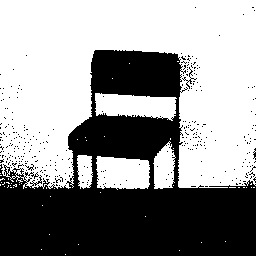
\includegraphics[width=0.2\textwidth]{img/res/e1a/alg1tipo1-chairga.jpg} &
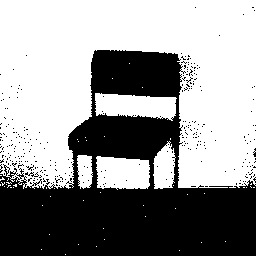
\includegraphics[width=0.2\textwidth]{img/res/e1a/alg1tipo6-chairga.jpg} &
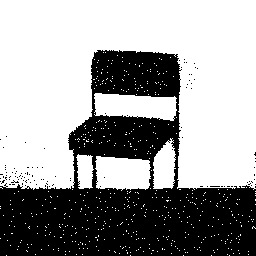
\includegraphics[width=0.2\textwidth]{img/res/e1a/alg1tipo6d0.75-chairga.jpg} &
\includegraphics[width=0.2\textwidth]{img/res/e1a/alg1tipo6d1.25-chairga.jpg} \\
\includegraphics[width=0.2\textwidth]{img/res/e1a/alg1tipo1-chairsp005.jpg} &
\includegraphics[width=0.2\textwidth]{img/res/e1a/alg1tipo6-chairsp005.jpg} &
\includegraphics[width=0.2\textwidth]{img/res/e1a/alg1tipo6d0.75-chairsp005.jpg} &
\includegraphics[width=0.2\textwidth]{img/res/e1a/alg1tipo6d1.25-chairsp005.jpg} \\
\includegraphics[width=0.2\textwidth]{img/res/e1a/alg1tipo1-chairsp020.jpg} &
\includegraphics[width=0.2\textwidth]{img/res/e1a/alg1tipo6-chairsp020.jpg} &
\includegraphics[width=0.2\textwidth]{img/res/e1a/alg1tipo6d0.75-chairsp020.jpg} &
\includegraphics[width=0.2\textwidth]{img/res/e1a/alg1tipo6d1.25-chairsp020.jpg} \\\hline
\end{tabular}
\caption{Umbrales para las imágenes con ruido con otras versiones de algoritmos.\label{tab:resultexp1imagenesruido}}
\end{table}

En relación con los errores con imagenes umbralizadas con otros algoritmos, no se obtiene ningún resultado concluyente ya que en ningún momento el error pasa de 0,1.

Además, se han hecho experimentos con imágenes con mucho y poco contraste. En este caso, la solución tenía el error de nuevo en un rango de diferencia de una décima, aunque permite llegar a opciones con mucho más bajo contraste que el algoritmo de la maximización de la entropía de Renyi, que es el que mejor lo hace entre los otros algoritmos presentados. En definitiva, con el algoritmo de maximización de la similitud se pueden llegar a segmentar imágenes con intervalos de menos de 15 niveles de gris. Se encuentra, también, el hechod de que en el caso de crear dos imágenes con alto y bajo contraste que sean ``contrarias'', la segmentación que se obtiene es la misma.


% EXPERIMENTO 2
\subsection{Experimento 2: busqueda del mejor umbral a través de funciones penalti\label{sec:exp2}}
\subsubsection{Explicación del experimento}
En vista del experimento anteior donde había momentos en los que la función de dombi no actuaba de forma correcta, se propone una nueva forma para poder elegir entre la función de Dombi o volver al método con la función REF. En concreto, se intentará dilucidar esta situación por medio de una función penalti. El proceso de la obtención del conjunto difuso cambiará, ya que no será una única función y tendrá el siguiente orden:
\begin{enumerate}
    \item Creación de todas las pertenencias con las 5 funciones REF presentadas y la función de Dombi con $w=1$.
    \item Agregación de todas las pertenencias anteriores con varias funciones, a saber:
        \begin{enumerate}
            \item Media aritmética.
            \item Media geométrica.
            \item Máximo.
            \item Mínimo.
            \item Integral Choquet.
            \item OWA de `al menos la mitad'. %\REV{nombre}
        \end{enumerate}
    \item Con todos estos resultados se actua con la función penalti para cada uno de los elementos $a_1,\dots a_n$ agregados y las pertenencias obtenidas en (1) $r=(r_1,\dots, r_m)$, obtendremos $p(a_i, r)=\sum_{j=1}^m \abs{a_i-r_j}$.
    \item Cogeremos como pertenencia aquel resultado de la agregación, $a_i$, que haga que el resultado de la función penalti sea máximo.
\end{enumerate}

En vista de que los resultados de la idea presentada anteriormente no presentaba a penas diferencia con el experimento 1. Por esta razón, en una segunda versión, se añadirá también la función de agregación siguiente con la intención de crear más {\em outlayers} que creen más posibles umbrales.
$$M_{zadeh}(r_1,\dots,r_m)=\max\left(0, \sum r-(n-1)\right)\cdot \sqrt[n]{\prod_{i=1}^n{r_i}}$$
Esta segunda versión son los resultados que se presentan a continuación.

\subsubsection{Resultados}

En la tabla \ref{tab:resultexp2agregado} se recogen los umbrales $t$ creados a través de la función penalti. De nuevo, en comparación con los presentados en la tabla \ref{tab:resultexp1otros} se puede observar que siempre son valores que se encuentran en el intervalo que pueden definir. Esto hace suponer que las imágenes tiene una umbralización correcta, algo que se puede comprobar con las imágenes del cuadro \ref{tab:resultexp2imagenagregado}. En relación al error (tabla \ref{tab:resultexp2agregado})sorprende la diferencia que existe frente

\begin{table}
\centering
\begin{tabular}{c|c|c|c|c}
\bb Silla&\bb Bloques&\bb Engranaje&\bb Letras&\bb Sombra\\\hline\hline
   127   &     68    &      92     &   196    &   123  \\\hline
\end{tabular}
\caption{Umbrales para cada imagen con el algoritmo 1 calculando la función de pertenencia a través de una función penalti.\label{tab:resultexp2agregado}}
\end{table}


\begin{table}
\centering
\begin{tabular}{ccccc}\hline
\includegraphics[width=0.15\textwidth]{img/res/e2a/alg1agregate-chair.jpg} &
\includegraphics[width=0.15\textwidth]{img/res/e2a/alg1agregate-block.jpg} &
\includegraphics[width=0.15\textwidth]{img/res/e2a/alg1agregate-02.jpg} &
\includegraphics[width=0.15\textwidth]{img/res/e2a/alg1agregate-09.jpg} &
\includegraphics[width=0.15\textwidth]{img/res/e2a/alg1agregate-07.jpg}\\\hline
\end{tabular}
\caption{Resultado para el nuevo algoritmo a través de penalti con todas las funciones propuestas.\label{tab:resultexp2imagenagregado}}
\end{table}


\begin{table}
\centering
\begin{tabular}{c|c|c|c|c}
\bb Bloques&\bb Engranaje&\bb Letras&\bb Sombra\\\hline\hline
     90,3727    &      124,9112     &     140,5241    &     194,3489  \\\hline
\end{tabular}
\caption{Errores en comparación con las imágenes segmentadas por el experto.\label{tab:erroresexp2agregado}}
\end{table}


Además, en la tabla \ref{tab:resultexp2agregadoruido} se pueden observar los umbrales obtenidos para las imágenes con ruido. De forma similar a las imágenes normales, el umbral vuelve a estar en el intervalo que se crea con los umbrales originales del experimento anterior. Tal y como se puede ver en la tabla \ref{tab:resultexp2imagenagregadoruido} el resultado para las imágenes con ruido gausiano y con ruido `sal y pimienta' con $p=0,05$ mientras que subiendo la probabilidad para el ruido, el umbral comienza a ser bastante inadecuado. Como es lógico, el ruido impulsivo no se consigue resolver aunque tampoco es así en el caso del gausiano, que segmenta de forma bastante adecuada aun no apreciandose un mínimo claro.

\begin{table}
\centering
\begin{tabular}{c|c|c}
\bb R. gausiano&\bb R. impulsivo 0.05&\bb R. impulsivo 0.2\\\hline\hline
   132   &     127    &      152    \\\hline
\end{tabular}
\caption{Umbrales para cada imagen ruido a través del algoritmo 1 calculando la función de pertenencia a través de una función penalti.\label{tab:resultexp2agregadoruido}}
\end{table}


\begin{table}
\centering
\begin{tabular}{ccc}\hline
\includegraphics[width=0.2\textwidth]{img/res/e2a/alg1agregate-chairga.jpg} &
\includegraphics[width=0.2\textwidth]{img/res/e2a/alg1agregate-chairsp005.jpg} &
\includegraphics[width=0.2\textwidth]{img/res/e2a/alg1agregate-chairsp020.jpg}\\\hline
\end{tabular}
\caption{Resultado para el nuevo algoritmo a través de penalti con todas las funciones propuestas para imágenes con ruido.\label{tab:resultexp2imagenagregadoruido}}
\end{table}



% EXPERIMENTO 3
\subsection{Experimento 3: sustitución de la función REF por la función de Dombi en el algoritmo para la obtenición del umbral óptimo}

\subsubsection{Explicación del experimento}
En este experimento se ha tomado el algoritmo de obtención del umbal óptimo maximizando la similitud (algoritmo 3A) para comprobar el efecto de la función de Dombi en él. Por esta razón, y en vista de los resultados del experimento 1, se plantean dos variantes. En primer lugar, se incorpora la función de dombi a las 5 funciones REF que ya estaban para poder ver qué umbral se obtiene, intentando escoger el mejor (algoritmo 3B). Después, se eligen los diferentes valores de $w$ que se han utilizado antes (algoritmo 3C). De esta forma, se intenta buscar cual de los umbrales calculados anteriormente de forma individual es el mejor.

\subsubsection{Resultados}

Hecho todo el cómputo, en la tabla \ref{tab:resultexp3dombi} se muestran los umbrales obtenidos tanto con el algoritmo original como por parte de las dos versiones que se han propuesto. Por un lado, es muy visible el hecho de que para la mayor parte de las imágenes la versión C no tiene utilidad, ya que elige umbrales totalmente fuera de la lógica. Por otra parte, se ve que la versión B es muy similar a la versión original. Esto hace pensar que esta versión podría hacer que las funciones de Dombi fueran interesantes para algunos casos. Los resultados gráficos se presentan en la tabla \ref{tab:resultexp3imagenesdombi}

\begin{table}
\centering
%\resizebox*{3\textwidth}{!}{
\begin{tabular}{c||c|c|c|c|c}
             &\bb Silla&\bb Bloques&\bb Engranaje&\bb Letras&\bb Sombra\\\hline\hline
\bb Alg. 3A  &   115   &    80    &     88      &    199   &    121   \\\hline
\bb Alg. 3B  &   127   &    123    &     84      &    200   &    125   \\\hline
\bb Alg. 3C  &   218   &    254    &     250     &    142   &    219   \\\hline
\end{tabular}
\caption{Umbrales para cada imagen con el algoritmo 3 en todas sus nuevas versiones.\label{tab:resultexp3dombi}}
\end{table}


\begin{table}
\centering
\begin{tabular}{cccccc}\hline
Alg. 3B\quad
\includegraphics[width=0.15\textwidth]{img/res/e3a/alg3btipo-chair.jpg} &
\includegraphics[width=0.15\textwidth]{img/res/e3a/alg3btipo-block.jpg} &
\includegraphics[width=0.15\textwidth]{img/res/e3a/alg3btipo-02.jpg} &
\includegraphics[width=0.15\textwidth]{img/res/e3a/alg3btipo-09.jpg} &
\includegraphics[width=0.15\textwidth]{img/res/e3a/alg3btipo-07.jpg}\\\hline
Alg. 3C\quad
\includegraphics[width=0.15\textwidth]{img/res/e3a/alg3ctipo-chair.jpg} &
\includegraphics[width=0.15\textwidth]{img/res/e3a/alg3ctipo-block.jpg} &
\includegraphics[width=0.15\textwidth]{img/res/e3a/alg3btipo-02.jpg} &
\includegraphics[width=0.15\textwidth]{img/res/e3a/alg3ctipo-09.jpg} &
\includegraphics[width=0.15\textwidth]{img/res/e3a/alg3ctipo-07.jpg}\\\hline
\end{tabular}
\caption{Resultado gráfico con el algoritmo 3 con las nuevas propuestas.\label{tab:resultexp3imagenesdombi}}
\end{table}

En cuanto al tiempo de cómputo, aunque crece con respecto a los algoritmos de los experimentos anteriores, este sigue estando en la misma media del algoritmo original, siempre que se tome como versión original la que definen las 5 REF del algoritmo 1. Todos los resultados gráficos son resumidos en la tabla \ref{tab:resultexp3imagenesdombi}.

%\REV{errores, imposible que sean esos...}

Para poder conocer cómo de buenos son los resultados, se comparan las imágenes obteniendo el error cuadrático medio (tabla\ref{tab:erroresexp3otros}). En esta se puede apreciar cómo se mantiene un error bastante similar con todos los algoritmos.

%\begin{table}
%\centering
%\begin{tabular}{c||c|c|c|c}
%                &\bb Bloques  &\bb Engranaje&\bb Letras  &\bb Sombra  \\\hline\hline
%\bb Alg. 3B     &   0,0082   &   124,9112   &   0,2019   &   0,1017   \\\hline
%\bb Alg. 3C     &     0      &   124,9112   &   0,0136   &   0,5744   \\\hline
%\end{tabular}
%\caption{Errores de las imágenes perfectas para cada imagen con el algoritmo 3 en todas sus versiones.\label{tab:erroresexp3dombi}}
%\end{table}


\begin{table}
\centering
\begin{tabular}{c||c|c|c|c}
                        &\bb Silla    &\bb Bloques  &\bb Engranaje &\bb Sombra    \\\hline\hline
\bb Alg. 3A (Original)  &   72,8822   &   93,8135   &   126,5836   &   124,7987   \\\hline
\bb Umb. Global         &   71,7070   &   81,0453   &   124,7637   &   122,4343   \\\hline
\bb {\em K-means}       &   71,7070   &   81,0453   &   124,9112   &   123,2863   \\\hline
\bb Método de Otsu      &   71,7070   &   81,0453   &   124,9112   &   123,2863   \\\hline
\bb Máx. Entropía Renyi &   56,9290   &   96,4543   &   121,5597   &   112,4747   \\\hline
\end{tabular}
\caption{Erorres de las imágenes obtenidas con otros algoritmos para cada imagen con el algoritmo 3 en todas sus versiones.\label{tab:erroresexp3otros}}
\end{table}


Se comprueba que las tendencias anteriores son también seguidas por aquellas imágenes que disponen de ruido. Es decir, la versión que se propone con la función de dombi con diferentes valores de $w$. También, los resultados con la versión B son más bajos con respecto a las versión original, algo que como se ha visto es bastante común desde el momento en el que se introducen las funciones de Dombi.


\begin{table}
\centering
\begin{tabular}{c||c|c|c}
        &\bb R. gausiano&\bb R. impulsivo 0.05&\bb R. impulsivo 0.2\\\hline\hline
\bb Alg. 3A  &   131   &    136    &     144      \\\hline
\bb Alg. 3B  &   128   &    127    &     127      \\\hline
\bb Alg. 3C  &   226   &    218    &     226      \\\hline
\end{tabular}
\caption{Umbrales para cada imagen ruidosa con el algoritmo 3 en todas sus versiones.\label{tab:resultexp3ruido}}
\end{table}



\begin{table}
\centering
\begin{tabular}{cccccc}\hline
Alg. 3B\quad
\includegraphics[width=0.18\textwidth]{img/res/e3a/alg3btipo-chairga.jpg} &
\includegraphics[width=0.18\textwidth]{img/res/e3a/alg3btipo-chairsp005.jpg} &
\includegraphics[width=0.18\textwidth]{img/res/e3a/alg3btipo-chairsp020.jpg}\\\hline
Alg. 3C\quad
\includegraphics[width=0.18\textwidth]{img/res/e3a/alg3ctipo-chairga.jpg} &
\includegraphics[width=0.18\textwidth]{img/res/e3a/alg3ctipo-chairsp005.jpg} &
\includegraphics[width=0.18\textwidth]{img/res/e3a/alg3ctipo-chairsp020.jpg}\\\hline
\end{tabular}
\caption{Representación gráfica del resultado .\label{tab:resultexp3imagenesruido}}
\end{table}


\begin{table}
\centering
\begin{tabular}{c||c|c|c}
        &\bb R. gausiano&\bb R. impulsivo 0.05&\bb R. impulsivo 0.2\\\hline\hline
\bb Alg. 3 Original     &   95,1075   &   66,4737   &   74,2907   \\\hline
\bb Umb. Global         &   94,8740   &   68,2635   &   77,5124   \\\hline
\bb {\em K-means}       &   95,1074   &   68,2635   &   77,5124   \\\hline
\bb Método de Otsu      &   94,8740   &   68,2635   &   77,5124   \\\hline
\bb Máx. Entropía Renyi &   85,9364   &   54,1976   &   65,7772   \\\hline
\end{tabular}
\caption{Errores para cada imagen ruidosa con otros algoritmos tomando como referencia la versión 3B.\label{tab:erroresexp3ruido}}
\end{table}



\subsection{Repetición de los experimentos con la corrección oportuna.}\label{sec:cambiodombi}
Vistos los resultados de los experimentos anteriores, y en especial el que se refiere al experimento 3, se plantea el porqué se obtiene un resultado tan malo. Este hecho es extraño sobre todo por el hecho de que a través de los diferentes valores de $w$, el algoritmo 1 con las funciones de dombi siempre tiene buenos resultados. Se comprueba el vector de similitudes que se obtiene para dilucidar qué umbral escoger en el algoritmo 3, lo que muestra que la similitud mayor no se encuentra en el mejor umbral. %\REV{¿ejemplo?}

Reestudiando la situación, se encuentra que en las propiedades de las funciones que propone Dombi (Lema \ref{def:propiedadesdombi}) se ha omitido que una función de equivalencia $e$ cumple $e(x,x)=1$. En particular, las funciones REF son un ejemplo de esta situación. La razón por la que no se puede cumplir esta propiedad es porque existe otra que dice $e(x,n(x))=0$. Como es evidente, el intentar mantener ambas a la vez es una contradicción. Por esta razón, el autor dice que sus funciones cumplirán en parte ambas en función de un parámetro. Esto hace que para dos elementos iguales no tengamos como resultado 1.

Vista la situación y sabiendo que la construcción que se utiliza para los conjuntos difusos hace necesario que la condición anterior se cumpla de forma plena, se intenta reescribir la función de pertenencia a los conjuntos difusos. De esta forma, se aplica a todos los experimentos que se han mostrado anteriormente esta nueva función (ecuación \ref{eq:intentodesolucionardombi})

\begin{equation}\label{eq:intentodesolucionardombi}
    \mu_{Q_t}(q)=\left\{ \begin{split}
                 \min\left( 1, \frac
                    {\unmedio \left(1+\left(1-\frac{2q}{L-1}\right)\left(1-\frac{2m_b}{L-1}\right)\right)}
                    {\unmedio \left(1+\left(1-\frac{2m_b}{L-1}\right)\left(1-\frac{2m_b}{L-1}\right)\right)}\right)
                 \text{\quad si\quad} q\leq t\\
                 \min\left( 1, \frac
                    {\unmedio \left(1+\left(1-\frac{2q}{L-1}\right)\left(1-\frac{2m_o}{L-1}\right)\right)}
                    {\unmedio \left(1+\left(1-\frac{2m_o}{L-1}\right)\left(1-\frac{2m_o}{L-1}\right)\right)}\right)
                \text{\quad si\quad} q > t
                \end{split}\right.
\end{equation}



%RESULTADOS DE LA REESCRITURA
\subsubsection{Resultados}
La opción que se ha propuesto anteriormente ha tenido resultados muy malos, de hecho, mucho peores que las presentadas en las secciones anteirores. Por esa razón y únicamente a modo de ejemplo, en las tablas \ref{tab:resultexp1bdombi} y \ref{tab:resultexp3bdombi} se pueden ver algunos resultados obtenidos. Este algoritmo, es por tanto, desechado de forma completa. Se acaba concluyendo que las funciones de Dombi no pueden sustituir directamente a funciones REF tal y como el autor sugería. Por esta razón, la umbralización con los métodos anteriores presentará resultados hetereogéneos lo que hace que no sea un método útil para su utilización habitual.

\begin{table}\begin{center}
%\resizebox*{3\textwidth}{!}{
\begin{tabular}{cc||c|c|c|c|c}
                                    &                   &\bb Silla&\bb Bloques&\bb Engranaje&\bb Letras&\bb Sombra\\\hline\hline
\bb{\multirow{2}{1.75cm}{$w=0,1$}}  &  \bb Umbral ($t$) &   234   &     8     &      0      &   157    &   250  \\
                                    &  \bb Tiempo (s)   &  0,002  &   0,675   &    0,686    &  0,689   &  0,688 \\\hline
\bb\multirow{2}{1.75cm}{$w=0,5$}    &  \bb Umbral ($t$) &   226   &     8     &     111     &   207    &   254  \\
                                    &  \bb Tiempo (s)   &  0,002  &   0,649   &    1,093    &  1,233   &  1,13  \\\hline
\bb\multirow{2}{1.75cm}{$w=0,75$}   &  \bb Umbral ($t$) &   226   &     8     &     122     &   182    &   238  \\
                                    &  \bb Tiempo (s)   &  0,002  &   0,677   &    0,686    &  0,688   &  0,679 \\\hline
\bb\multirow{2}{1.75cm}{$w=1$}      &  \bb Umbral ($t$) &   226   &     8     &      90     &   191    &   246  \\
                                    &  \bb Tiempo (s)   &  0,002  &   0,63    &    0,642    &  0,646   &  0,642 \\\hline
\bb\multirow{2}{1.75cm}{$w=1,25$}   &  \bb Umbral ($t$) &   226   &     8     &     250     &   203    &   252  \\
                                    &  \bb Tiempo (s)   &  0,002  &   0,682   &    0,684    &  0,688   &  0,686 \\\hline
\bb\multirow{2}{1.75cm}{$w=1,5$}    &  \bb Umbral ($t$) &   242   &     6     &     250     &   213    &   254  \\
                                    &  \bb Tiempo (s)   &  0,002  &   0,666   &    1,106    &  1,246   &  1,138 \\\hline
\bb\multirow{2}{1.75cm}{$w=2$}      &  \bb Umbral ($t$) &   250   &     3     &     250     &   215    &    66  \\
                                    &  \bb Tiempo (s)   &  0,002  &   0,631   &    0,640    &  0,644   &  0,641 \\\hline
\bb\multirow{2}{1.75cm}{$w=5$}      &  \bb Umbral ($t$) &   250   &     1     &     250     &   254    &    66  \\
                                    &  \bb Tiempo (s)   &  0,002  &   0,657   &    0,671    &  0,672   &  0,673 \\\hline
\end{tabular}\end{center}
\caption{Umbrales y tiempo de cómputo para cada imagen con el algoritmo 1 reescrito a través de funciones de Dombi.\label{tab:resultexp1bdombi}}
\end{table}

\begin{table}\begin{center}
\begin{tabular}{c||c|c|c}
    &\bb Ruido gausiano&\bb Ruido impulsivo 0.05&\bb Ruido impulsivo 0.2\\\hline\hline
\bb Alg. 3A &   131   &    136    &     144     \\\hline
\bb Alg. 3B &   131   &    234    &     152     \\\hline
\bb Alg. 3C &   254   &    234    &     250    \\\hline
\end{tabular}\end{center}
\caption{Umbrales para versión del algoritmo 3 reescrito con imágenes ruidosas.\label{tab:resultexp3bdombi}}
\end{table}

\end{document}
